\section{مقدمه}
هدف از این تمرین، بهبود پردازنده‌ی تک‌چرخه‌ای طراحی‌شده در تمرین 5 و تبدیل کردن آن به یک پردازنده‌ی خط لوله‌ی (\lr{Pipeline}) پنج مرحله‌ای است. در معماری خط لوله، چندین دستور به‌طور هم‌زمان در مراحل مختلف پردازش قرار می‌گیرند و توان عملیاتی سیستم به‌طور چشم‌گیری افزایش می‌یابد. همچنین این هم‌پوشانی پدیده‌‌ی \lr{Hazards} را ایجاد می‌کند که در این تمرین با دو روش ارسال رو به جلو (\lr{Forwarding}) و توقف (\lr{Stall}) برطرف می‌شوند.

پنج زیرماژول تمرین پنجم (واحد کنترل (\lr{\code{control\_unit}})، بانک ثبات (\lr{\code{regfile}})، واحد حساب و منطق (\lr{\code{alu}})، ضرب‌کننده (\lr{\code{multiplier}}) و تقسیم‌کننده (\lr{\code{divider}})) بدون هیچ تغییری استفاده شدند. تمام منطق جدید خط لوله، شامل ثبات‌های واسط، تشخیص و رفع مخاطرات داده و کنترلی، در ماژول سطح بالا (\lr{\code{main}}) پیاده‌سازی شده است.

\section{مراحل خط لوله و ثبات‌های واسط}
پردازنده از پنج مرحله‌ی پشت سر هم تشکیل شده است: واکشی دستور (\lr{Fetch, F})، رمزگشایی (\lr{Decode, D})، اجرا (\lr{Execute, E})، دسترسی به حافظه (\lr{Memory, M}) و بازنویسی (\lr{Write Back, W}). در هر لبه‌ی بالارونده‌ی ساعت، محتوای چهار ثبات واسط (\lr{\code{FD}}، \lr{\code{DE}}، \lr{\code{EM}} و \lr{\code{MW}}) به‌روزرسانی می‌شود. هر ثبات واسط یک بیت اعتبار (\lr{\code{Valid}}) دارد که در صورت صفر بودن، دستور موجود در آن مرحله به‌عنوان \lr{NOP} در نظر گرفته می‌شود. این بیت برای تمام ثبات‌ها هنگام \lr{Reset} صفر می‌شود. فیلدهای ذخیره‌شده در هر ثبات واسط در این جدول آمده است:

\begin{table}[H]
    \centering
    \caption{ثبات‌های واسط خط لوله و فیلدهای آن‌ها}
    \vspace{0.2cm}
    \begin{tabular}{|c|p{10.5cm}|}
        \hline
        \textbf{ثبات واسط} & \textbf{فیلدهای ذخیره‌شده}                                                                                                                                                                                                                                                                                                                    \\
        \hline
        \lr{\code{FD}}     & \lr{\code{Valid}},\ \lr{\code{PC}},\ \lr{\code{Instr}}                                                                                                                                                                                                                                                                                       \\
        \hline
        \lr{\code{DE}}     & \lr{\code{Valid}},\ \lr{\code{PC}},\ \lr{\code{Instr}},\ \lr{\code{RsVal}},\ \lr{\code{RtVal}},\ \lr{\code{Imm}} (\lr{sign extended}),\ \lr{\code{WriteReg}},\ \lr{\code{RegWrite}},\ \lr{\code{MemRead}},\ \lr{\code{MemWrite}},\ \lr{\code{Branch}},\ \lr{\code{MemtoReg}},\ \lr{\code{ALUControl}},\ \lr{\code{ALUSrc}},\ \lr{\code{Jal}} \\
        \hline
        \lr{\code{EM}}     & \lr{\code{Valid}},\ \lr{\code{PC}},\ \lr{\code{Instr}},\ \lr{\code{ALUResult}},\ \lr{\code{RtVal}},\ \lr{\code{WriteReg}},\ \lr{\code{RegWrite}},\ \lr{\code{MemRead}},\ \lr{\code{MemWrite}},\ \lr{\code{MemtoReg}},\ \lr{\code{Jal}}                                                                                                       \\
        \hline
        \lr{\code{MW}}     & \lr{\code{Valid}},\ \lr{\code{PC}},\ \lr{\code{ALUResult}},\ \lr{\code{ReadData}},\ \lr{\code{WriteReg}},\ \lr{\code{RegWrite}},\ \lr{\code{MemtoReg}},\ \lr{\code{Jal}}                                                                                                                                                                     \\
        \hline
    \end{tabular}
\end{table}

ثبات شمارنده‌ی برنامه (\lr{\code{PC}}) به صورت \lr{Word Index} است، یعنی در هر چرخه‌ی عادی یک واحد افزایش می‌یابد (\lr{\code{pc\_plus\_1 = PC + 1}}) و مستقیماً به خروجی \lr{\code{InstrAddr}} متصل شده. آدرس داده نیز از رابطه‌ی \lr{\code{DataAddr = EM\_ALUResult >> 2}} به دست می‌آید (چون رجیسترها آدرس‌های بایتی نگه می‌دارند). منطق تعیین مقدار بعدی \lr{\code{PC}} نیز با یک مالتی‌پلکسر چهارحالته پیاده‌سازی شده است:

\vspace{0.2cm}
\begin{latin}
    \begin{lstlisting}[language=Verilog]
wire [31:0] next_pc = branch_taken ? branch_target :
                      jump_in_D    ? jump_target   :
                      stall        ? PC            :
                      pc_plus_1;
    \end{lstlisting}
\end{latin}
\vspace{0.2cm}

پرش شرطی فعال (\lr{\code{branch\_taken}}) بالاترین اولویت را دارد، پس از آن پرش غیرشرطی (\lr{\code{jump\_in\_D}})، و بعد از آن توقف خط لوله (\lr{\code{stall}}) که \lr{\code{PC}} را ثابت نگه می‌دارد، و در غیر این صورت افزایش عادی \lr{\code{pc\_plus\_1}} است. در ادامه نحوه‌ی محاسبه‌ی این سیگنال‌ها و سازوکار کلی رفع مخاطرات توضیح داده می‌شود.

\section{مدیریت مخاطرات داده}

\subsection{تشخیص مخاطره و مکانیزم توقف}
اولین گام برای تشخیص \lr{Hazard} این است که مشخص کنیم آیا دستور در حال رمزگشایی (مرحله‌ی \lr{D}) به ثبات‌های \lr{\code{rs}} یا \lr{\code{rt}} نیاز دارد یا خیر. برای این منظور دو سیگنال ترکیبی \lr{\code{uses\_rs}} و \lr{\code{uses\_rt}} بر اساس \lr{\code{opcode}} و \lr{\code{funct}} دستور جاری در ثبات \lr{\code{FD}} تعریف شده‌اند:

\vspace{0.2cm}
\begin{latin}
    \begin{lstlisting}[language=Verilog]
wire uses_rs = FD_Valid && (
    (FD_opcode == RTYPE && (FD_funct == F_ADD || FD_funct == F_SUB ||
                            FD_funct == F_MUL || FD_funct == F_DIV || FD_funct == F_JR)) ||
    (FD_opcode == ADDI) || (FD_opcode == SUBI) ||
    (FD_opcode == LW) || (FD_opcode == SW) ||
    (FD_opcode == BEQ));

wire uses_rt = FD_Valid && (
    (FD_opcode == RTYPE && (FD_funct == F_ADD || FD_funct == F_SUB ||
                            FD_funct == F_MUL || FD_funct == F_DIV)) ||
    (FD_opcode == SW) || (FD_opcode == BEQ));
    \end{lstlisting}
\end{latin}
\vspace{0.2cm}

در گام بعد، با بررسی ثبات‌های واسط \lr{\code{DE}} و \lr{\code{EM}}، مشخص می‌شود که آیا دستور قرار گرفته در مرحله‌ی E یا M قرار است در ثباتی بنویسد که دستور D به آن وابسته است یا خیر:

\vspace{0.2cm}
\begin{latin}
    \begin{lstlisting}[language=Verilog]
wire e_will_write = DE_Valid && DE_RegWrite && DE_WriteReg != 5'd0;
wire m_will_write = EM_Valid && EM_RegWrite && EM_WriteReg != 5'd0;

assign data_hazard = FD_Valid && (
    (uses_rs && e_will_write && DE_WriteReg == FD_rs) ||
    (uses_rs && m_will_write && EM_WriteReg == FD_rs) ||
    (uses_rt && e_will_write && DE_WriteReg == FD_rt) ||
    (uses_rt && m_will_write && EM_WriteReg == FD_rt));
    \end{lstlisting}
\end{latin}

هرگاه \lr{\code{data\_hazard}} فعال شود، سیگنال \lr{\code{stall}} بالا می‌رود و دو اتفاق به صورت موازی رخ می‌دهند: ثبات \lr{\code{FD}}، \lr{Freeze} می‌شود تا دستور مخاطره‌دار در مرحله‌ی \lr{D} بماند، و در همان حال یک \lr{Bubble} با صفر کردن \lr{\code{DE\_Valid}} به مرحله‌ی \lr{E} تزریق می‌شود. نکته‌ی مهم این است که ثبات \lr{\code{DE}} به‌جای منجمد شدن، حباب دریافت می‌کند. اگر \lr{\code{DE}} منجمد می‌شد، دستور مخاطره‌ساز برای چرخه‌های بعد همچنان در مرحله‌ی \lr{E} باقی می‌ماند، سیگنال \lr{\code{e\_will\_write}} مدام فعال می‌ماند و \lr{\code{data\_hazard}} هرگز صفر نمی‌شد و یک توقف بی‌نهایت رخ می‌داد. با تزریق حباب، دستور مخاطره‌ساز به‌طور طبیعی به مراحل بعدی پیش می‌رود و سیگنال‌های \lr{\code{e\_will\_write}} و \lr{\code{m\_will\_write}} در طول چرخه‌های بعدی صفر می‌شوند.

تعداد چرخه‌های توقف به جایگاه دستور تولیدکننده بستگی دارد: اگر آن دستور در مرحله‌ی \lr{E} باشد، دو چرخه توقف لازم است تا نتیجه‌اش به مرحله‌ی \lr{W} برسد و بتواند در دسترس قرار گیرد. اگر در مرحله‌ی \lr{M} باشد، یک چرخه کافی است.

\subsection{ارسال رو به جلو از مرحله‌ی \lr{W} به \lr{D}}
برای کاهش تعداد توقف‌های لازم، یک مسیر ارسال رو به جلو از مرحله‌ی \lr{W} به مرحله‌ی \lr{D} پیاده‌سازی شده است. اگر دستوری که در حال بازنویسی در مرحله‌ی W است (ثبات \lr{\code{MW}}) در همان ثباتی بنویسد که دستور در \lr{D} به آن نیاز دارد، مقدار محاسبه‌شده مستقیماً ارسال می‌شود و نیازی به خواندن از بانک ثبات نیست:

\vspace{0.2cm}
\begin{latin}
    \begin{lstlisting}[language=Verilog]
wire [31:0] d_rs_val =
    (MW_Valid && MW_RegWrite && MW_WriteReg == FD_rs && FD_rs != 5'd0)
    ? MW_WriteData : reg_rs_data;
wire [31:0] d_rt_val =
    (MW_Valid && MW_RegWrite && MW_WriteReg == FD_rt && FD_rt != 5'd0)
    ? MW_WriteData : reg_rt_data;
    \end{lstlisting}
\end{latin}
\vspace{0.2cm}

مقدار \lr{\code{MW\_WriteData}} به‌صورت ترکیبی محاسبه می‌شود: برای \lr{\code{JAL}} آدرس بازگشت، برای \lr{\code{LW}} داده‌ی خوانده‌شده از حافظه، و برای سایر دستورها نتیجه‌ی \lr{ALU}. اگرچه بانک ثبات سنکرون است و در همان لبه‌ای که \lr{\code{MW\_Valid}} بالا می‌رود می‌نویسد، همچنان به این مسیر نیاز داریم چون خواندن ترکیبی بانک ثبات هنوز مقدار قدیمی پیش از آن لبه را می‌بیند.

نکته‌ی مهم: بانک ثبات در این پیاده‌سازی از روی سیگنال‌های ثبات \lr{\code{EM}} (نه \lr{\code{MW}}) نوشته می‌شود:

\vspace{0.2cm}
\begin{latin}
    \begin{lstlisting}[language=Verilog]
wire [31:0] em_write_data =
    EM_Jal              ? ((EM_PC + 32'd1) << 2) :
    (EM_MemtoReg==2'b01)? DataIn                 :
    EM_ALUResult;

regfile rf(.RegWrite(EM_RegWrite && EM_Valid),
           .WriteReg(EM_WriteReg),
           .WriteData(em_write_data), ...);
    \end{lstlisting}
\end{latin}
\vspace{0.2cm}

دلیل این است که تست‌بنچ بلافاصله پس از فعال‌شدن \lr{\code{W\_Valid}} مقادیر ثبات‌ها را بررسی می‌کند. چون نوشتن بانک ثبات و لچ شدن \lr{\code{EM}} به \lr{\code{MW}} هر دو \lr{Non-blocking} هستند و روی همان لبه‌ی ساعت رخ می‌دهند، در لحظه‌ی \lr{posedge + $\varepsilon$} هر دو تکمیل شده‌اند. اگر بازنویسی از روی سیگنال‌های \lr{\code{MW}} انجام می‌شد، یک چرخه دیرتر از \lr{\code{MW\_Valid}} رخ می‌داد و تمام دستورات در تست‌بنچ شکست می‌خوردند.

در نهایت، مقادیر \lr{\code{d\_rs\_val}} و \lr{\code{d\_rt\_val}} هنگام پیشروی دستور از \lr{D} به \lr{E} در ثبات‌های \lr{\code{DE\_RsVal}} و \lr{\code{DE\_RtVal}} ذخیره می‌شوند و در مرحله‌ی \lr{E} توسط \lr{ALU} و ماژول‌های ضرب/تقسیم استفاده می‌گردند.

\subsection{توقف برای دستورات \lr{MUL} و \lr{DIV}}
ماژول‌های ضرب و تقسیم هر کدام به 32 کلاک نیاز دارند. در این مدت سیگنال \lr{\code{mul\_div\_stall}} فعال می‌ماند تا این کارها انجام شود: ثبات \lr{\code{FD}} منجمد می‌شود تا دستورات جدید وارد خط لوله نشوند، و ثبات \lr{\code{DE}} نیز منجمد می‌شود تا عملوندهای \lr{\code{MUL}}/\lr{\code{DIV}} در طول محاسبه بدون تغییر باقی بمانند. برخلاف توقف‌های مخاطره‌ی داده، در اینجا منجمد کردن \lr{\code{DE}} کاملاً صحیح است، چون دستور \lr{\code{MUL}}/\lr{\code{DIV}} خودش باید در مرحله‌ی \lr{E} بماند تا محاسبه به اتمام برسد، نه اینکه یک دستور دیگر جایش را بگیرد. این توقف با سیگنال \lr{\code{mul\_div\_stall}} از سیگنال \lr{\code{data\_hazard}} جدا نگه داشته شده تا در بلوک به‌روزرسانی ثبات‌ها بتوان رفتار متفاوتی برای هر کدام تعریف کرد.

\section{مدیریت مخاطرات کنترلی}

\subsection{پرش‌های غیرشرطی در مرحله‌ی \lr{D}}
دستورات \lr{\code{J}}، \lr{\code{JAL}} و \lr{\code{JR}} در مرحله‌ی \lr{D} شناسایی می‌شوند، چون مقصد پرش آن‌ها مستقیماً از فیلدهای دستور یا ثبات‌های رمزگشایی‌شده قابل محاسبه است و نیازی به واحد \lr{ALU} ندارد:

\vspace{0.2cm}
\begin{latin}
    \begin{lstlisting}[language=Verilog]
assign jump_in_D = FD_Valid && !stall &&
    ((FD_opcode == J) || (FD_opcode == JAL) ||
     (FD_opcode == RTYPE && FD_funct == F_JR));

assign branch_taken = DE_Valid && DE_Branch && zero && !mul_div_stall;

wire flush_FD = jump_in_D || branch_taken;
    \end{lstlisting}
\end{latin}
\vspace{0.2cm}

شرط \lr{\code{!stall}} در تعریف \lr{\code{jump\_in\_D}} برای دستور \lr{\code{JR}} اهمیت ویژه‌ای دارد: اگر ثباتی که \lr{\code{JR}} به آن پرش می‌کند هنوز در راه باشد (مخاطره‌ی داده)، ابتدا باید توقف رخ دهد تا مقدار صحیح در \lr{\code{d\_rs\_val}} آماده شود، و تنها بعد از آن \lr{\code{jump\_in\_D}} فعال گردد.

مقصد پرش بسته به نوع دستور متفاوت است. برای \lr{\code{J}} و \lr{\code{JAL}}، آدرس ۲۶ بیتی فیلد دستور مستقیماً به‌عنوان شاخص کلمه‌ای استفاده می‌شود (\lr{\code{jump\_target = \{6'b0, FD\_jaddr\}}}). برای \lr{\code{JR}}، مقدار ثبات که یک آدرس بایتی است به شاخص کلمه‌ای تبدیل می‌شود (\lr{\code{jump\_target = d\_rs\_val >> 2}}).

هر پرش غیرشرطی دستوری را که بلافاصله پس از آن \lr{fetch} شده باطل می‌کند. این کار با فعال‌شدن \lr{\code{flush\_FD}} انجام می‌شود که فقط \lr{\code{FD\_Valid}} را صفر می‌کند. خود دستور پرش (مثلاً \lr{\code{JAL}}) بدون هیچ تغییری از \lr{D} به \lr{E} و سپس به \lr{W} پیشروی می‌کند تا بازنویسی در ثبات در مرحله‌ی W انجام شود. از آنجا که \lr{\code{JAL}} باید آدرس بایتی دستور بعد از خودش را در \lr{\code{\$31}} ذخیره کند و \lr{\code{PC}} شاخص کلمه‌ای است، مقدار ذخیره‌شده برابر \lr{\code{(EM\_PC + 1) << 2}} است (همان \lr{\code{em\_write\_data}} در حالت \lr{\code{Jal=1}})؛ و ثبات مقصد در مرحله‌ی D صریحاً برابر \lr{\code{\$31}} تنظیم می‌شود:
\[
    \text{\lr{\code{DE\_WriteReg}}} = \text{\lr{\code{Jal}}} \;?\; 31 \;:\; \bigl(\text{\lr{\code{RegDst}}} \;?\; \text{\lr{\code{FD\_rd}}} \;:\; \text{\lr{\code{FD\_rt}}}\bigr)
\]

\subsection{پرش شرطی (\lr{BEQ}) در مرحله‌ی \lr{E}}
دستور \lr{\code{BEQ}} باید در مرحله‌ی E شناسایی شود، چون بررسی برابری دو ثبات به سیگنال \lr{\code{Zero}} از خروجی واحد \lr{ALU} نیاز دارد که تنها در این مرحله در دسترس است. به همین دلیل، مخاطره‌ی کنترلی آن یک مرحله دیرتر از پرش‌های غیرشرطی تشخیص داده می‌شود. هنگامی که \lr{\code{branch\_taken}} فعال می‌شود، دو اقدام موازی انجام می‌گیرد: \lr{\code{flush\_FD}} فعال می‌شود تا دستوری که در آن لحظه در مرحله‌ی D است (و از مسیر اشتباه آمده) باطل شود، و \lr{\code{DE\_Valid}} نیز در همان چرخه صفر می‌شود تا یک حباب به مرحله‌ی E تزریق گردد.

آدرس هدف پرش در مرحله‌ی \lr{E} از رابطه‌ی زیر محاسبه می‌شود:
\[
    \text{\lr{\code{branch\_target}}} = (\text{\lr{\code{DE\_PC}}} + 1) + \text{\lr{\code{DE\_Imm}}}
\]
که در آن \lr{\code{DE\_PC}} شاخص کلمه‌ای دستور \lr{\code{BEQ}} است و \lr{\code{DE\_Imm}} مقدار \lr{offset}ِ \lr{sign-extend} شده است که مستقیماً به‌صورت تعداد کلمه استفاده می‌شود.

نکته‌ی طراحی مهم این است که خود دستور \lr{\code{BEQ}} نباید در مرحله‌ی E یا M باطل شود. تست‌بنچ برای تأیید اجرای هر دستور منتظر می‌ماند تا \lr{\code{W\_Valid}} فعال و \lr{\code{W\_PC}} برابر آدرس آن دستور شود؛ بنابراین \lr{\code{BEQ}} باید بدون هیچ تغییری تا مرحله‌ی W پیش برود، هرچند که هیچ بازنویسی‌ای در ثبات‌ها ندارد.

\section{اجرای آزمون}
این کد را با تست‌بنچ داده شده بررسی کردیم و نتیجه‌ی آن به این صورت می‌باشد:

\begin{figure}[H]
    \centering
    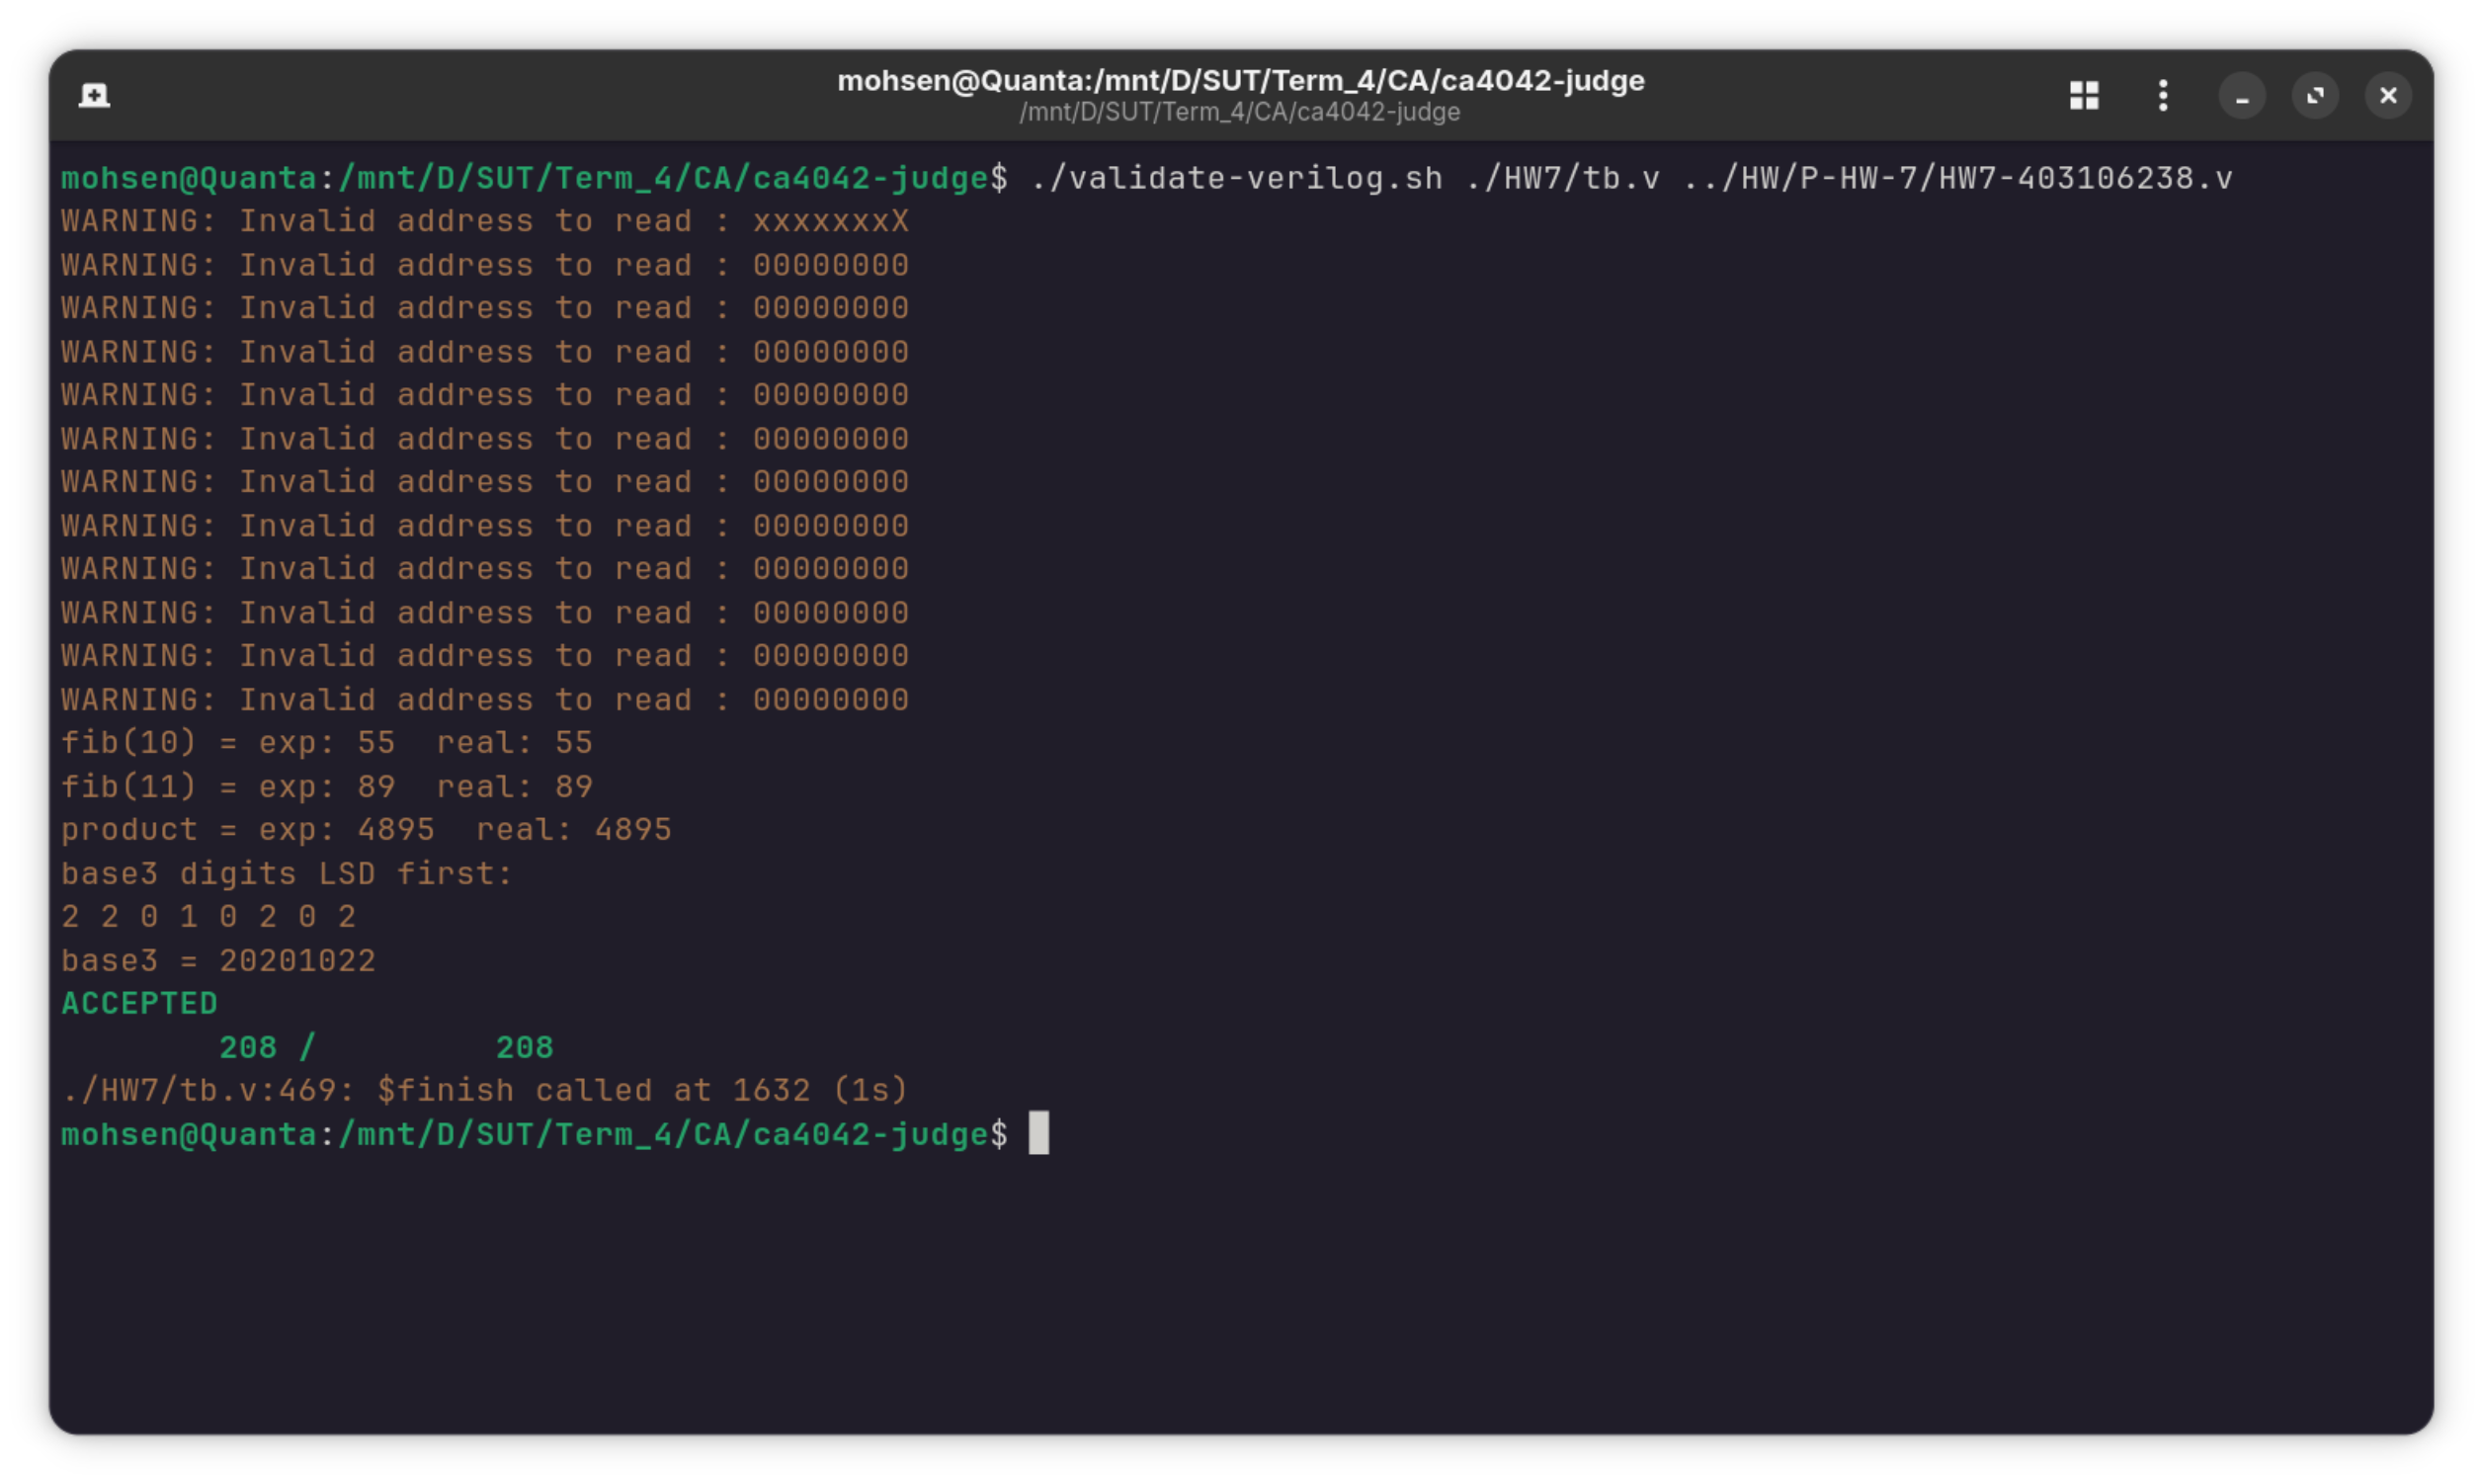
\includegraphics[width=1.0\textwidth]{assets/test_result.png}
    \caption{اجرای تست‌بنچ تمرین}
\end{figure}